
\section{Casi d'uso}
\subsection{Scopo}
L'obbiettivo di questa sezione è quello di presentare e descrivere tutti i casi d'uso, individuati dal team, in riferimento alle funzionalità richieste nell'applicazione.
\subsection{Attori}
Non essendo richiesto nessun tipo di servizio di autenticazione o più in generale una distinzione gerarchica degli utenti, è presente un solo attore nella gerarchia ovvero: l'utente generico.
\begin{figure}[h!]
    \centering
    
\includegraphics[scale=0.50]{../../assets/Utente.png}
    \caption{Gerarchia attori}
\end{figure}

\subsection{UC1 - Caricamento dataset}
\begin{figure}[h!]
    \centering
    % Sistema immagine inserendo tag UC e abbelliscila dc
    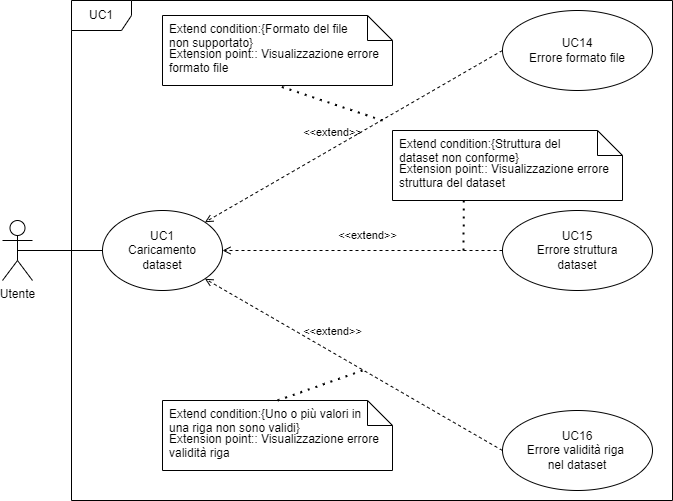
\includegraphics[scale=0.50]{../../assets/Caricamento_dataset.png}
    \caption{UC1 - Caricamento dataset}
\end{figure}
\begin{itemize}
    \item \textbf{Attore primario:} Utente.
    \item \textbf{Precondizioni:} Il sistema è funzionante
    \item \textbf{Postcondizioni:} Viene visualizzato un messaggio che avvisa l'utente del corretto caricamento dei dati e della loro validità. 
                                   I dati vengono caricati nel sistema
    \item \textbf{Scenario principale:}
          \begin{enumerate}
              \item L'utente seleziona il file da caricare
              \item L'utente carica il file
          \end{enumerate}
    \item \textbf{Estensioni:}
    \begin{itemize}
        \item   Nel caso in cui l'utente carichi un file in un formato non supportato
                \begin{enumerate}
                    \item I dati non vengono caricati
                    \item Viene visualizzato un messaggio di errore esplicativo [\hyperref[sec:UC - Errore formato file]{UC}] % To Do: metti il link alla sezione   
                \end{enumerate}
        \item   Nel caso in cui l'utente carichi un file non correttamente strutturato
                \begin{enumerate}
                    \item I dati non vengono caricati
                    \item Viene visualizzato un messaggio di errore esplicativo [\hyperref[sec:UC - Errore struttura dataset]{UC}]
                \end{enumerate}
        \item   Nel caso in cui i dati di una o più righe non siano validi
                \begin{enumerate}
                    \item Viene visualizzato un messaggio di errore esplicativo [\hyperref[sec:UC - Errore validita riga]{UC}] % To Do: metti il link alla sezione
                \end{enumerate}
    \end{itemize} 
\end{itemize}

% --------------------------------------------------------------------
% SCELTA TIPO GRAFICO
% --------------------------------------------------------------------

\subsection{UC2 - Scelta tipologia grafico}
\label{sec:UC2}
\begin{figure}[h!]
    \centering
    % Controlla che UC abbia il numero corretto
    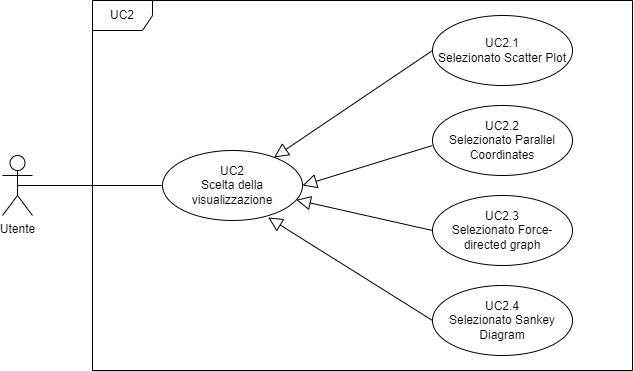
\includegraphics[scale=0.50]{../../assets/Selezione_tipo_grafico.png}
    \caption{UC2 - Scelta tipologia grafico}
\end{figure}
\begin{itemize}
    \item \textbf{Attore primario}: Utente.
    \item \textbf{Precondizioni}: Il dataset è stato caricato correttamente.
    \item \textbf{Postcondizioni}: Viene mostrata la visualizzazione scelta.
    \item \textbf{Scenario principale}:
          \begin{enumerate}
              \item L'utente seleziona il tipo di grafico da visualizzare tra le tipologie disponibili.
          \end{enumerate}
    \item \textbf{Generalizzazioni}:
    \begin{itemize}
        \item L'utente seleziona una delle seguenti opzioni:
                \begin{enumerate}
                    \item \textit{Scatter Plot} \hyperref[sec:UC2.1]{UC2.1}.
                    \item \textit{Parallel Coordinates} \hyperref[sec:UC2.2]{UC2.2}.
                    \item \textit{Force-directed Graph} \hyperref[sec:UC2.3]{UC2.3}.
                    \item \textit{Sankey Diagram} \hyperref[sec:UC2.4]{UC2.4}.
                \end{enumerate}
    \end{itemize} 
\end{itemize}

\subsubsection{UC2.1 - Selezionato Scatter Plot}
\label{sec:UC2.1}
\begin{itemize}
    \item \textbf{Attore primario}: Utente.
    \item \textbf{Precondizioni}: Il dataset è stato caricato correttamente [UC2].
    \item \textbf{Postcondizioni}: Viene mostrata la visualizzazione \textit{Scatter Plot} scelta dall'utente con possibilità di selezionare il numero di dimensioni significative \hyperref[sec:UC2]{UC?} e personalizzare lo stile \hyperref[sec:UC2]{UC?}. %inserire il numero corretto dello stile e delle dimensioni
    \item \textbf{Scenario principale}:
          \begin{enumerate}
              \item L'utente seleziona il grafico \textit{Scatter Plot} e il sistema ritorna tale grafico con conseguente possibilità di personalizzazione. 
          \end{enumerate}
\end{itemize}

\subsubsection{UC2.2 - Selezionato Parallel Coordinates}
\label{sec:UC2.2}
\begin{itemize}
    \item \textbf{Attore primario}: Utente.
    \item \textbf{Precondizioni}: Il dataset è stato caricato correttamente [UC2].
    \item \textbf{Postcondizioni}: Viene mostrata la visualizzazione \textit{Parallel Coordinates} scelta dall'utente con possibilità di selezionare il numero di dimensioni significative \hyperref[sec:UC2]{UC?} e personalizzare lo stile \hyperref[sec:UC2]{UC?}. %inserire il numero corretto dello stile e delle dimensioni
    \item \textbf{Scenario principale}:
          \begin{enumerate}
              \item L'utente seleziona il grafico \textit{Parallel Coordinates} e il sistema ritorna tale grafico con conseguente possibilità di personalizzazione. 
          \end{enumerate}
\end{itemize}

\subsubsection{UC2.3 - Selezionato Force-directed Graph}
\label{sec:UC2.3}
\begin{itemize}
    \item \textbf{Attore primario}: Utente.
    \item \textbf{Precondizioni}: Il dataset è stato caricato correttamente [UC2].
    \item \textbf{Postcondizioni}: Viene mostrata la visualizzazione \textit{Force-directed Graph} scelta dall'utente con possibilità di selezionare il numero di dimensioni significative \hyperref[sec:UC2]{UC?} e personalizzare lo stile \hyperref[sec:UC2]{UC?}. %inserire il numero corretto dello stile e delle dimensioni
    \item \textbf{Scenario principale}:
          \begin{enumerate}
              \item L'utente seleziona il grafico \textit{Force-directed Graph} e il sistema ritorna tale grafico con conseguente possibilità di personalizzazione. 
          \end{enumerate}
\end{itemize}

\subsubsection{UC2.4 - Selezionato Sankey Diagram}
\label{sec:UC2.4}
\begin{itemize}
    \item \textbf{Attore primario}: Utente.
    \item \textbf{Precondizioni}: Il dataset è stato caricato correttamente [UC2].
    \item \textbf{Postcondizioni}: Viene mostrata la visualizzazione \textit{Sankey Diagram} scelta dall'utente con possibilità di selezionare il numero di dimensioni significative \hyperref[sec:UC2]{UC?} e personalizzare lo stile \hyperref[sec:UC2]{UC?}. %inserire il numero corretto dello stile e delle dimensioni
    \item \textbf{Scenario principale}:
          \begin{enumerate}
              \item L'utente seleziona il grafico \textit{Sankey Diagram} e il sistema ritorna tale grafico con conseguente possibilità di personalizzazione. 
          \end{enumerate}
\end{itemize}

% --------------------------------------------------------------------
% SEZIONE ERRORI
% --------------------------------------------------------------------

\subsection{UC - Errore formato file}
\label{sec:UC - Errore formato file}
\begin{itemize}
    \item \textbf{Attore primario:} Utente
    \item \textbf{Precondizioni:} L'utente carica un file in un formato non supportato.
    \item \textbf{Postcondizioni:} L'utente visualizza un messaggio di errore e il file non viene caricato.
    \item \textbf{Scenario principale:}
          \begin{enumerate}
              \item L'utente visualizza un messaggio di errore esplicativo
              \item L'utente clicca "OK" per proseguire.
          \end{enumerate}
\end{itemize}

\subsection{UC - Errore struttura dataset}
\label{sec:UC - Errore struttura dataset}
\begin{itemize}
    \item \textbf{Attore primario:} Utente
    \item \textbf{Precondizioni:} L'utente carica un file nel formato supportato ma che non è correttamente strutturato  
                                  (e.g. due o più colonne sono invertite oppure una o più colonne sono mancanti). 
    \item \textbf{Postcondizioni:} L'utente visualizza un messaggio di errore e il file non viene caricato.
    \item \textbf{Scenario principale:}
          \begin{enumerate}
              \item L'utente visualizza un messaggio di errore esplicativo.
              \item L'utente clicca "OK" per proseguire.
          \end{enumerate} 
\end{itemize}
\subsection{UC - Errore validità riga nel dataset}
\label{sec:UC - Errore validita riga}
\begin{itemize}
    \item \textbf{Attore primario:} Utente
    \item \textbf{Precondizioni:} L'utente carica un file nel formato supportato e ben strutturato ma, una o più righe presentano
                                  un dato non valido (e.g. nella colonna relativa ai \textit{timestamp} il valore è negativo).  
    \item \textbf{Postcondizioni:} L'utente visualizza un messaggio di errore che chiede o di ignorare la riga non valida, 
                                   oppure di continuare.
    \item \textbf{Scenario principale:}
    \begin{itemize}
        \item   L'utente sceglie di ignorare la riga
                \begin{enumerate}
                    \item L'utente visualizza un messaggio di errore esplicativo.
                    \item L'utente clicca "IGNORA" per ignorare la riga non valida.
                    \item Il file viene caricato escludendo la riga precedentemente ignorata.
                \end{enumerate} 
        \item   L'utente sceglie di proseguire.
                \begin{enumerate}
                    \item L'utente visualizza un messaggio di errore esplicativo.
                    \item L'utente clicca "OK" per proseguire.
                    \item Il file non viene caricato.
                \end{enumerate} 
    \end{itemize}
\end{itemize}


\subsection{UC7 - Personalizzazione visiva dei grafici}
\begin{figure}[h!]
	\centering
	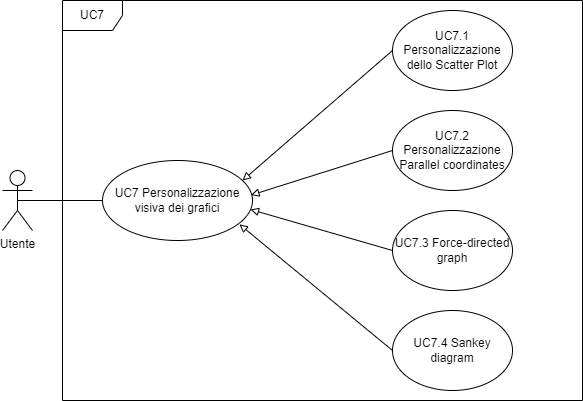
\includegraphics[scale=0.60]{../../assets/personalizzazioneVisivaGrafici.drawio.png}
	\caption{UC7 - Personalizzazione visiva dei grafici}
\end{figure}
\begin{itemize}
	\item \textbf{Attore primario:} Utente.
	\item \textbf{Precondizioni:} L'utente ha scelto uno di grafici a disposizione nell'interfaccia [UC2].
	\item \textbf{Postcondizioni:} 
	Il grafico viene ridisegnato secondo le scelte selezionate dall'utente.
	\item \textbf{Scenario principale:}
	L'utente seleziona il tipo di grafico e i colori che desidera e, per ogni elemento cambiato, i valori di default del grafico
    vengono cambiati. Nel caso si scelta di tornare nella vista di defauslt, le modifiche eseguite torneranno ai valori standard.
    \item \textbf{Generalizzazioni}:
    \begin{itemize}
        \item L'utente seleziona una delle seguenti opzioni:
                \begin{enumerate}
                    \item \textit{Personalizza Scatter Plot} \hyperref[sec:UC7.1]{UC7.1}.
                    \item \textit{Personalizza Parallel Coordinates} \hyperref[sec:UC7.2]{UC7.2}.
                    \item \textit{Personalizza Force-directed Graph} \hyperref[sec:UC7.3]{UC7.3}.
                    \item \textit{Personalizza Sankey Diagram} \hyperref[sec:UC7.4]{UC7.4}.
                \end{enumerate}
    \end{itemize} 
\end{itemize}
\subsubsection{UC7.1 - Personalizzazione Scatter plot}
\label{sec:UC7.1}
\begin{figure}[h!]
	\centering
	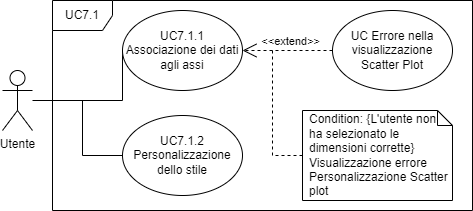
\includegraphics[scale=0.90]{../../assets/personalizzazioneScatterPlot.drawio.png}
	\caption{UC7 - Personalizzazione Scatter Plot}
\end{figure}
\begin{itemize}
    \item \textbf{Attore primario:} Utente.
	\item \textbf{Precondizioni:} L'utente ha scelto il grafico scatter plot. \hyperref[sec:UC2.1]{UC2.1}.
	\item \textbf{Postcondizioni:} 
	Il grafico viene ridisegnato secondo le scelte selezionate dall'utente.
	\item \textbf{Scenario principale:}L'utente decide:
	\begin{itemize}
        \item Associazione delle dimensioni agli assi \hyperref[sec:UC7.1.1]{UC7.1.1}.
        \item Personalizzazione dello stile \hyperref[sec:UC7.1.2]{UC7.1.2}.
    \end{itemize}
\end{itemize}
\paragraph{UC7.1.1 - Associazione delle dimensioni agli assi}
\label{sec:UC7.1.1}
    \begin{itemize}
        \item \textbf{Attore primario:} Utente.
        \item \textbf{Precondizioni:} L'utente ha selezionato lo scatter plot \hyperref[sec:UC2.1]{UC2.1}.
	    \item \textbf{Postcondizioni:} L'utente ha associato le dimensioni disponibili con gli assi del grafico.
	    \item \textbf{Scenario principale:} L'utente sceglie quali dimensioni associare agli assi del grafico.
	    \item \textbf{Estensioni:} Nel caso l'utente non abbia associato correttamente le dimensioni agli assi del grafico:
              \begin{itemize}
                  \item Non viene visualizzato nessun grafico.
                  \item Viene visualizzato un errore di personalizzazione grafico.
              \end{itemize}
    \end{itemize}
\paragraph{UC7.1.2 - Personalizzazione dello stile}
\label{sec:UC7.1.2}
    \begin{itemize}
        \item \textbf{Attore primario:} Utente.
        \item \textbf{Precondizioni:} L'utente ha selezionato lo scatter plot \hyperref[sec:UC2.1]{UC2.1}.
	    \item \textbf{Postcondizioni:} L'utente ha selezionato tra le opzioni disponibili lo stile che preferisce.
	    \item \textbf{Scenario principale:} L'utente visualizza le opzioni di colori per la personalizzazione di ogni specifica del grafico, nel caso l'utente non li modifichi rimangono quelli di default.
    \end{itemize}

\subsubsection{UC7.2 - Personalizzazione Parallel coordinates}
\label{sec:UC7.2}
\begin{figure}[h!]
	\centering
	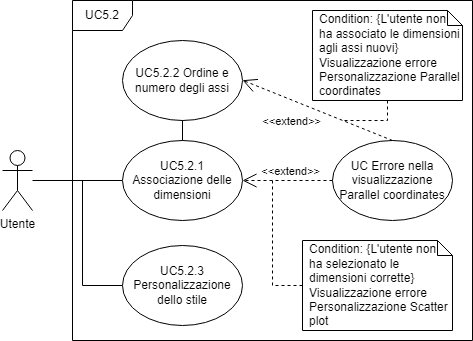
\includegraphics[scale=0.90]{../../assets/personalizzazioneParallelCoordinates.drawio.png}
	\caption{UC7 - Personalizzazione Parallel coordinates}
\end{figure}
\begin{itemize}
    \item \textbf{Attore primario:} Utente.
	\item \textbf{Precondizioni:} L'utente ha scelto il grafico Parallel coordinates. \hyperref[sec:UC2.1]{UC2.1}.
	\item \textbf{Postcondizioni:} Il grafico viene ridisegnato secondo le scelte selezionate dall'utente.
	\item \textbf{Scenario principale:}L'utente decide:
	\begin{itemize}
        \item Associazione delle dimensioni \hyperref[sec:UC7.2.1]{UC7.2.1}.
        \item Ordine degli assi \hyperref[sec:UC7.2.2]{UC7.2.2}.
        \item Personalizzazione dello stile \hyperref[sec:UC7.2.3]{UC7.2.3}.
    \end{itemize}
\end{itemize}
\paragraph{UC7.2.1 - Associazione delle dimensioni}
\label{sec:UC7.2.1}
    \begin{itemize}
        \item \textbf{Attore primario:} Utente.
        \item \textbf{Precondizioni:} L'utente ha selezionato Parallel coordinates. \hyperref[sec:UC2.2]{UC2.2}.
	    \item \textbf{Postcondizioni:} L'utente ha associato le dimensioni disponibili con gli assi del grafico.
	    \item \textbf{Scenario principale:} L'utente sceglie quali dimensioni associare agli assi del grafico.
	    \item \textbf{Estensioni:} Nel caso l'utente non abbia associato correttamente le dimensioni agli assi del grafico:
              \begin{itemize}
                  \item Non viene visualizzato nessun grafico.
                  \item Viene visualizzato un errore di visualizzazione personalizzazione grafico.
              \end{itemize}
    \end{itemize}
\paragraph{UC7.2.2 - Ordine e numero degli assi}
\label{sec:UC7.2.2}
    \begin{itemize}
        \item \textbf{Attore primario:} Utente.
        \item \textbf{Precondizioni:} L'utente ha selezionato Parallel coordinates. \hyperref[sec:UC2.2]{UC2.2}.
	    \item \textbf{Postcondizioni:} L'utente ha deciso un ordine degli assi e il loro numero.
	    \item \textbf{Scenario principale:} L'utente sceglie ordine e numero degli assi.
	    \item \textbf{Estensioni:} Nel caso l'utente abbia creato nuovi assi ma non abbai associato nessuna dimensione con essi:
              \begin{itemize}
                  \item Non viene visualizzato nessun grafico.
                  \item Viene visualizzato un errore di visualizzazione personalizzazione grafico.
              \end{itemize}
    \end{itemize}
\paragraph{UC7.2.3 - Personalizzazione dello stile}
\label{sec:UC7.2.3}
    \begin{itemize}
        \item \textbf{Attore primario:} Utente.
        \item \textbf{Precondizioni:} L'utente ha selezionato Parallel coordinates \hyperref[sec:UC2.2]{UC2.2}.
	    \item \textbf{Postcondizioni:} L'utente ha selezionato tra le opzioni disponibili lo stile che preferisce.
	    \item \textbf{Scenario principale:} L'utente visualizza le opzioni di colori per la personalizzazione di ogni specifica del grafico, nel caso l'utente non li modifichi rimangono quelli di default.
    \end{itemize}

\subsubsection{UC7.3 - Personalizzazione Force-directed graph}
\label{sec:UC7.3}
\subsubsection{UC7.4 - Personalizzazione Sankey diagram}
\label{sec:UC7.4}


\subsection{UC8 - Visualizzazione di default dei grafici}
\begin{figure}[h!]
	\centering
	% Sistema immagine inserendo tag UC e abbelliscila dc
	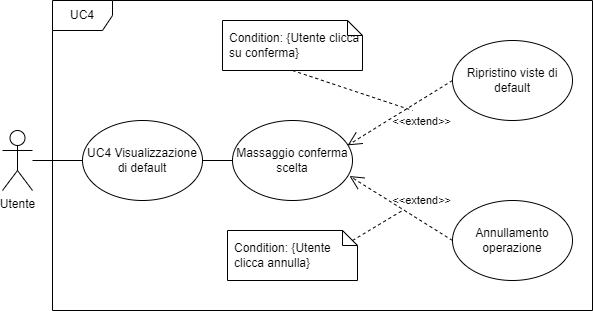
\includegraphics[scale=0.80]{../../assets/visualizzazione_default.png}
	\caption{UC8 - Visualizzazione di default dei grafici}
\end{figure}
\begin{itemize}
	\item \textbf{Attore primario:} Utente.
	\item \textbf{Precondizioni:} Il dataset è presente e caricato correttamente.
	\item \textbf{Postcondizioni:} 
	Vengono riportati i grafici alla visualizzazione di default.
	\item \textbf{Scenario principale:}
	\begin{itemize}
		\item   L'utente sceglie di ripristinare le viste
	\begin{enumerate}
		\item L'utente clicca sul pulsante di ripristino
		\item Viene visualizzato un messaggio di riconferma
		\item L'utente clicca "OK" per confermare la scelta
		\item I grafici vengono resettati alla vista di default
	\end{enumerate}
		\item   L'utente sceglie di annullare l'operazione
	\begin{enumerate}
		\item L'utente clicca sul pulsante di ripristino
		\item Viene visualizzato un messaggio di riconferma
		\item L'utente clicca "ANNULLA" per annullare l'operazione
		\item Ritorno alla vista corrente senza modifiche apportate
	\end{enumerate}	
	\end{itemize}
\end{itemize}